\documentclass[11pt]{article}

\usepackage{float}
\usepackage{hyperref}
\usepackage{graphicx}
% formatting
\usepackage{fullpage}
\usepackage{verbatim}
\usepackage{moreverb}
\usepackage{minted}
\usepackage{parskip}
\let\verbatiminput=\verbatimtabinput
\def\verbatimtabsize{4\relax}

\hypersetup{
  colorlinks=true,
  linkcolor=blue!50!red,
  urlcolor=green!70!black
}

\begin{document}
\title{EECS 151/251A FPGA Lab\\
Lab 1: Getting Set Up and Familiarizing Yourself with Tools}

\author{Prof. Jan Rabaey \\
TAs: George Alexandrov, Ali Moin \\Department of Electrical Engineering and Computer Sciences\\
College of Engineering, University of California, Berkeley}
\date{}
\maketitle

\section{Foreword}
All labs and and the project for this class will be done in groups of 2. This first lab is straightforward and serves as an introduction to the hardware and software we will be using throughout the class. Hence, you are free to work on it by yourself, but it is highly encouraged that you find a lab partner as soon as possible. Please talk to a TA if you need any help or if there are an odd number of students in your section.

\section{Setting Up Accounts}

\subsection{Course website and Piazza}
If you are enrolled in this class, you should have access to the EECS 151/251A home page (\url{https://bcourses.berkeley.edu/courses/1473222}) already. If you don't have access, please let a TA or the instructor know immediately so we can resolve the issue. You should also register for a Piazza account and enroll in the EECS 151/251A class as soon as possible (\url{https://piazza.com/class/jkdsruyfq2x2xv}). We will be using Piazza to make announcements and as a discussion forum for this class and for the labs. The course website lists helpful resources, the course outline, and material for lectures, labs, and homework.

\subsection{Getting an EECS 151 Account}
All students enrolled in the FPGA lab are required to get a EECS 151 class account to login to the workstations in lab. This semester, you can get a class account by using the webapp here:
\url{https://inst.eecs.berkeley.edu/webacct}

Once you login using your CalNet ID, you can click on 'Get a new account' in the eecs151 row. Once the account has been created, you can email your class account form to yourself to have a record of your account information.

Now you should be able to login to the workstations we have available in the lab. Enter your login and initial password in the login screen. Let the lab TA know if you have any problems setting up your class account.

\subsubsection{Changing your password}
To change your default password, click on Applications on the top left toolbar on your workstation desktop, then hover over System, then click on Terminal. In the terminal type and execute the command: \verb|ssh update.cs.berkeley.edu|

You can then follow the prompts to set up a new password. You can always use the same webapp that you used to create your account to reset your password if you forget it.

\subsection{Getting a Github Account}
If you haven't done so previously, sign up for a Github account at \url{https://github.com/} with your berkeley.edu email address.

If you already have a Github account that's registered with your personal email address, don't create a new account. Instead, login to Github, go here \url{https://github.com/settings/emails}, and add your berkeley.edu email address to your Github account.

Once you have an account, send the TAs an email with your Github account username and email and your class account login (eecs151-xxx). Our email addresses are gpalex@berkeley.edu and moin@berkeley.edu. Try to do this as soon as possible.

%\subsection{How to Login to the Lab Workstations From Your Laptop}

\section{Getting Familiar with our Development Environment}
\subsection{Linux Basics}
In this class, we will be using a Linux development environment. We will be using CentOS as our Linux distro, which is a free version of Red Hat Linux. If you are unfamiliar or uncomfortable with Linux, and in particular, using the bash terminal, you should definitely check out this tutorial:

\url{https://www.digitalocean.com/community/tutorial_series/getting-started-with-linux}

It is highly recommended to go through all four parts of the tutorial above, even if you already are familiar with the content. To complete the labs and projects for this course, you will find it helpful to have good command line skills.

One of the best ways to expand your working knowledge of bash is to watch others who are more experienced. Pay attention when you are watching someone else's screen and ask questions when you see something you don't understand. You will quickly learn many new commands and shortcuts.

\subsection{Git Basics}
Version control systems help track how files change over time and make it easier for collaborators to work on the same files and share their changes. For projects of any reasonable complexity, some sort of version control is an absolute necessity. There are tons of version control systems out there, each with some pros and cons. In this class, we will be using Git, one of the most popular version control systems. It is highly recommended that you make the effort to really understand how Git works, as it will make understanding how to actually use it much easier. Please check out the following link, which provides a good high level overview:

\url{http://git-scm.com/book/en/Getting-Started-Git-Basics}

Once you think you understand the material above, please complete the following tutorial:

\url{http://try.github.com}

Git is a very powerful tool, but it can be a bit overwhelming at first. If you don't know what you are doing, you can really cause lots of headaches for yourself and those around you, so please be careful. If you are ever doubtful about how to do something with Git ask a TA or an experienced classmate.

For the purposes of this class you will probably only need to be proficient with the following commands:
\begin{itemize}
\item {\tt git status}
\item {\tt git add}
\item {\tt git commit}
\item {\tt git pull}
\item {\tt git push}
\item {\tt git clone}
\end{itemize}
However, if you put in the effort to learn how to use some of the more powerful features (diff, blame, branch, log, mergetool, rebase, and many others), they can really increase your productivity.

Git has a huge feature set which is well documented on the internet. If there is something you think Git should be able to do, chances are the command already exists. We highly encourage you to explore and discuss with fellow classmates and TA's.

\textit{Optional:} If you would like to explore further, check out the slightly more advanced tutorial written for CS250:

\url{http://inst.eecs.berkeley.edu/~cs250/fa13/handouts/tut1-git.pdf}

\section{Setting Up Github Access}
We will be using Github as our remote Git server for this class. Github is a popular Git hosting service which is home to many private and public (open-source) projects.

\subsection{SSH Keys}
Github authenticates you for access to your repository using ssh keys. Follow this tutorial to get SSH keys set up (this should be done on a lab workstation when you are logged in with your eecs151 class account).

First, create a new SSH key (do this on the lab computer):
\begin{verbatim}
ssh-keygen -t rsa -b 4096 -C "your_email@berkeley.edu"
\end{verbatim}
Keep hitting enter to use the default settings.

Then, from your terminal run:
\begin{verbatim}
cat ~/.ssh/id_rsa.pub
\end{verbatim}

Copy the public key that's printed out in its entirety. Go here: \url{https://github.com/settings/keys}, click on 'New SSH Key', paste your public key into the box, and click 'Add SSH key'.

Finally test your SSH connection: \url{https://help.github.com/articles/testing-your-ssh-connection/#platform-linux}.

If you have any issues, ask a TA for help.

\subsection{Acquiring Lab Files}
The lab files, and eventually the project files, will be made available through a git repository provided by the staff. The suggested way to obtain these files is as follows. First, set up your ssh keys as described above. Then run the command below in your home directory,

\begin{verbatim}
git clone git@github.com:EECS150/fpga_labs_fa18.git
\end{verbatim}

Whenever a new lab is released, you should only need to do a \verb|git pull| to retrieve the new files. Furthermore, if there are any updates to the labs, \verb|git pull| will fetch the changes and merge them in.

For now, you will only have pull access to this repository. If you make any local commits, you will not be able to push them to the remote server. Later on, each team will receive their own private repo for the project, and you will be able to push and pull from that.

\section{Our Development Platform - Xilinx Pynq-Z1}
For the labs in this class, we will be using the Xilinx Pynq-Z1 development board which is built on the Zynq development platform. Our development board is a printed circuit board that contains a Zynq-7000 FPGA along with a host of peripheral ICs and connections. The development board makes it easy to program the FPGA and allows us to experiment with different peripherals.

The best reference for this board is provided by Digilent: \url{https://reference.digilentinc.com/reference/programmable-logic/pynq-z1/reference-manual} (a PDF version of this manual is available in the \verb|fpga_labs_fa18/resources| folder). Browse the documentation there to get a feel for both what features the board has and, more importantly, what information the documentation has, should you need it later.

Being a development board, the silkscreen print clearly identifies connectors of interest. You should have used the most basic IO features in the last lab: GPIO LEDs, slide switches, and push-buttons. You should also be familiar with other basic elements of the board: input power socket, power switch, and the USB programming port. The following image identifies important parts of the board that may not have been obvious:

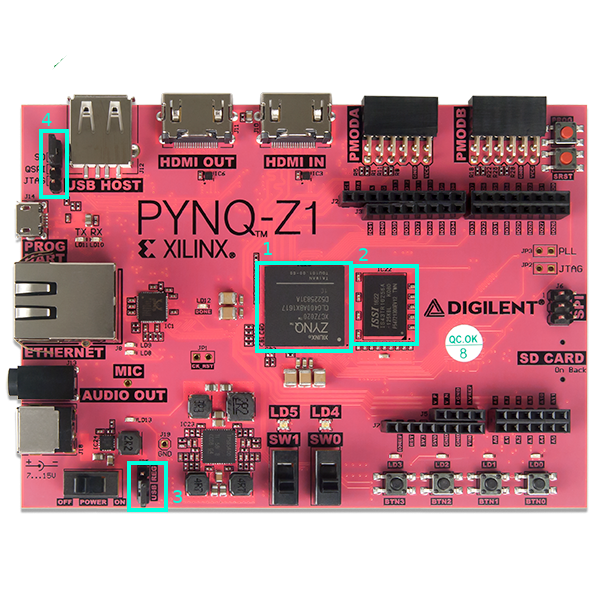
\includegraphics[width=\textwidth]{figs/z1_top_annotated.png}
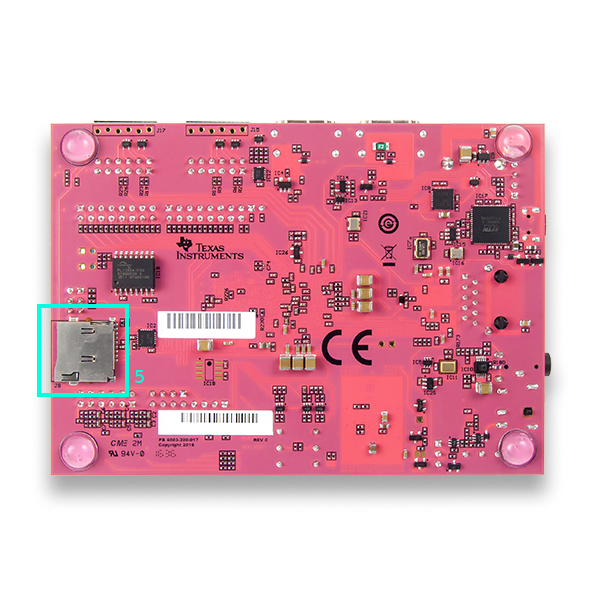
\includegraphics[width=\textwidth]{figs/z1_bottom_annotated.png}
\begin{enumerate}
	\item Zynq 7000-series FPGA. It is connected to the peripheral ICs and I/O connectors via PCB traces.
	\item ISSI DRAM chip
	\item Power source jumper: shorting "REG" has the board use the external power adapter as a power source; shorting "USB" has it rely on the 5 V provided by USB. The latter will work unless your design needs to power a lot of external peripherals. Since we have labs and power adaptors available, we avoid this.
	\item Programming mode jumper
	\item SD card slot
\end{enumerate}

\section{The FPGA - Xilinx Zynq-7000 7z020}
To help you become familiar with the FPGA that you will be working with through the semester, please skim Chapter 21: Programmable Logic Description of the \href{https://www.xilinx.com/support/documentation/user_guides/ug585-Zynq-7000-TRM.pdf}{Technical Reference Manual} and Chapter 2 of the \href{http://www.xilinx.com/support/documentation/user_guides/ug474_7Series_CLB.pdf}{Xilinx 7-series Configurable Logic Block User Guide}. Pay particular attention to pages 15-25 on Slices and pages 40-42 on Multiplexers. Answer the following questions (you should be able to discuss your answers for checkoff):

\subsection{Checkoff Questions}
\begin{enumerate}
	\item How many SLICEs are in a single CLB?
	\item How many inputs do each of the LUTs on a Zynq-7000 FPGA have?
	\item How many LUTs does the 7z020 have?
	\item How do you implement logic functions of 7 inputs in a single SLICEL? How about 8? Draw a high-level circuit diagram to show how the implementation would look. Be specific about the elements (LUTs, muxes) that are used.
	\item What is the difference between a SLICEL and a SLICEM?
\end{enumerate}

\section{Overview of the FPGA Build Toolchain}

Before we begin the lab, we should familiarize ourselves with the CAD (computer aided design) tools that translate HDL (Verilog) into a working circuit on the FPGA. These tools will pass your design through several stages, each one bringing it closer to a concrete implementation. In previous years, older evaluation platforms (the ML505) used older FPGAs (a Xilinx Virtex-5 LX110T) and an older software suite (Xilinx ISE). Although there was a GUI, we had Makefiles to invoke each subsequent program in the toolchain to carry out the complete synthesis and perform analysis.

Our new boards use Xilinx's updated design software, the Vivado Design Suite. Vivado emphasizes its powerful integrated scripting capabilities (using the Tcl language) and integration with other high-level design tools (such as, for example, High-Level Synthesis - but more on that later). It also has support for equivalent Makefiles and automation through Tcl. The GUI itself has the disadvantage of being very manual to work with. Repeatedly changing and running parameters quickly becomes tedious. Our eventual goal is definitely to automate the design process as much as possible. For learning, however, the GUI has the invaluable property of guiding us through each step of the process. Read through the following sections but don't worry about the details for now. We will run through the entire tool flow on a simple project at the end of this lab.

\subsection{Synthesis}

To run the synthesis step in the Vivado Design Suite (that is, turn your HDL into combinational and sequential logic), select \emph{Run Synthesis} in the \emph{Flow Navigator} pane to the left other interface. If this has been run before, the synthesized design can be inspected by selecting \emph{Open Synthesized Design}.

\subsection{Implementation}

The implementation step in the Vivado GUI is equivalent to the translation, mapping and place and route steps in the manual pipeline. Again, this takes the logical circuit synthesized previously and maps it to the physical logic devices our particular FPGA actually has. Select \emph{Run Implementation} in the \emph{Flow Navigator} to run it, then select \emph{Open Implementation} to inspect its outputs.

\subsection{Xilinx Design Constraints (XDC)}

How do we connect one of our signals to a physical device? How do we specify special properties of the circuit that might matter for correctness and timing? The Xilinx Design Constraints file (with the \verb|.xdc| extension) specifies necessary properties of the design (just like the old User Constraints File), and is a crucial input to the implementation phase. XDC is inspired by the Synopsis ASIC synthesis toolchain and aims to be somewhat compatible. You are writing a form of TCL for the Vivado TCL interpreter. More information can be found on page 22 of the \href{https://www.xilinx.com/support/documentation/sw_manuals/xilinx2015_2/ug911-vivado-migration.pdf}{Vivado migration guide}.

Take a look at this snippet from the XDC inside \verb|lab1/lab1.srcs/constrs_1/new/z1top.xdc|:

\begin{minted}{tcl}
set_property -dict { PACKAGE_PIN L19   IOSTANDARD LVCMOS33 } [get_ports { BUTTONS[3] }];
\end{minted}

This syntax assigns the properties \verb|PACKAGE_PIN| and \verb|IOSTANDARD| with the values \verb|L19| and \verb|LVCMOS33| (respectively) to the port \verb|BUTTONS[3]|, a signal we defined in our Verilog source. Each of these properties has a separate consequence in the synthesis process:

\begin{itemize}
\item The pin to which the \verb|BUTTONS[3]| signal should be connected to the physical pin L19 on the FPGA package.
\item The logic convention (maximum voltage, what ranges constitute low and high, etc) for that port will be LVCMOS33.
\end{itemize}

\subsection{Bitstream generation}

To generate the programming file our FPGA will understand, we invoke \emph{Generate Bitstream} in the \emph{Flow Navigator}.

\subsection{Timing Analysis}

A timing analysis report can be generated under \emph{Synthesis} in \emph{Flow Navigator}, by expanding \emph{Open Synthesized Design} and selecting \emph{Report Timing Summary}.

\subsection{Design Reports}

Reports are automatically generated at each step in the build flow. You should be able to discover them under each of the expanded stages in the \emph{Flow Navigator}. The \emph{Project Summary} window (under the \emph{Window} menu) presents a nice summary of the reports generated through each step. You will see some examples later in the lab.

\subsection{Programming the FPGA}

To send the bitstream to the FPGA with the Vivado GUI, we have to use the \emph{Hardware Manager}. This is accessible under \emph{Program and Debug} in the \emph{Flow Navigator}, right under \emph{Generate Bitstream}. Once connected to your FPGA over the USB JTAG interface, you can select \emph{Program Device} in the \emph{Flow Navigator} (or in the \emph{Hardware Manager} pane that opens) to perform the programming.

\subsection{Toolchain Conclusion}
This section was information dense. Don't worry about understanding the internals of each tool and the exact file formats they work with, especially for different Xilinx software generations. Just understand what each step of the toolchain does at a high level and you will be good for this class. You will use these kinds of tools regularly, but for now let the staff worry about making sure they work in the first place.

\section{Your First FPGA Design}
Finally, let's conclude with a simple example of a complete project. Throughout the semester, you will build increasingly complex designs using Verilog, a widely used hardware description language (HDL). For this lab, you will use basic Verilog to describe a simple digital circuit.

Now that you have cloned the \verb|fpga_labs_fa18| repository, you can \verb|cd| to the 
\verb|fpga_labs_fa18/lab1| directory to see this lab's skeleton files. You will note that there is a \verb|lab1.srcs| directory and a \verb|lab1.xpr| file.

Past versions of this course used an FPGA development toolchain from the Xilinx ISE Design Suite. The modern alternative, and that which we are now using for this course, is the Xilinx Vivado Design Suite (``Vivado'' for short). We will initially use Vivado's Integrated Development Environment (IDE) instead of any command-line tools, though you will eventually see that the framework (especially with Pynq) is ripe for automation with TCL and Python scripting.

The lab skeleton files include the project meta data file, \verb|.xpr|, a Verilog source file for a simple top-level module, \verb|z1top.v|, and a constraints file, \verb|z1top.xdc|.

HDL source files like \verb|z1top.v| (where the HDL is Verilog) describe the circuit that you want to create on the FPGA. \verb|z1top.v| describes a circuit that is the \emph{top-level} of your circuit: it has access to the signals that come into and out of the FPGA chip. Constraints files, such as \verb|z1top.xdc|, allow the engineer (you!) to tailor specific properties of the synthesized design to how they wish to use their specific chip. This includes the crucial mapping between FPGA input/output pins and signal names used in circuit descriptions. We'll cover more on constraints files in the next lab, so don't worry about the details too much just yet.

\subsection{Set up your Pynq-Z1}

\begin{enumerate}
  \item Plug in the power adaptor to provide mains power.
  \item Insert the factory-imaged SD card to provide a boot OS for the onboard ARM (mostly for use later).
  \item Connect the USB interface to a spare USB port on your workstation.
  \item Turn the board on.
\end{enumerate}

\subsection{Open the Lab 1 project in the Vivado Design Suite}

In our Centos environment, press Alt-F2 to bring up a command dialog. Type the full path to the \verb|vivado| binary to execute it:

\begin{verbatim}
/opt/Xilinx/Vivado/current/bin/vivado
\end{verbatim}

(You can also run this from a terminal or create a Desktop shortcut.)

Once in Vivado, open up the \verb|lab1/lab1.xpr| project file. Look around the environment to try and get a feel for the GUI. Open up the \verb|lab1/lab1.srcs/sources_1/new/z1top.v| source file. Again, this file contains a Verilog module description which specifies which signals are inputs into the module and which signals are outputs.

The \verb|BUTTONS| input is a signal that is 4 bits wide (as indicated by the [3:0] width descriptor). This input signal represents the logic signals coming from the momentary push-button switches on the bottom right side of your Pynq-Z1 board. You should inspect your board to find these switches and confirm that there are 4 of them. Another basic input signal is \verb|SWITCHES|, which is 2 bits wide (as indicated by the [1:0] descriptor). Each of these two signals represents the slide switches on the Pynq-Z1, located just to the left of the momentary switches (look for SW0 and SW1).

The \verb|LEDS| output is a signal that is 6 bits wide (as indicated by the [5:0] width descriptor). This output signal represents the logic signals coming out of the FPGA and going into the bank of LEDs at the bottom right of the Pynq-Z1, just above the buttons. Almost. There are only 4 LEDs there; 2 more are tri-color LEDs located just above the slide switches in the middle.

In this file, we can describe how the slide switches, push buttons and LEDs are connected through the FPGA. There is one line of code that describes an AND gate that takes the values of one of the buttons and one of the slide switches, ANDs them together, and sends that signal out to the first LED. Let's put this digital circuit on the FPGA!

\subsection{Synthesize and Program}

\begin{enumerate}
  \item In Vivado, locate the \emph{Flow Navigator} pane to the left of the screen. Near the bottom, under \emph{Program and Debug}, click \emph{Generate Bitstream}. Accept the default settings and wait. This should invoke the dependent steps in the flow: \emph{Synthesis} and \emph{Implementation} (among other things).
    \begin{itemize}
      \item Selecting \emph{Project Manager} will give you a nice overview of the progress of various background steps while this happens.
      \item So will watching the \emph{Messages} and \emph{Logs} output.
    \end{itemize}
  \item When the synthesis and bitstream generation is done, select \emph{Open Hardware Manager} and connect to your FPGA.
    \begin{itemize}
      \item If you haven't before, or the hardware manager says no devices are connected, select \emph{Menu} $\rightarrow$ \emph{Open New Target}
      \item You should see \verb|xilinx_tcf| listed under Harware Targets in the top pane. In the bottom pane, two entries: \verb|arm_dap_0| and \verb|xc7z020_1|. That's good. \emph{Next} $\rightarrow$ \emph{Finish}.
    \end{itemize}
  \item Back in the \emph{Flow Navigator} on the left, under \emph{Program and Debug}, select \emph{Program Device}. The only option to program will be the FPGA, \verb|xc7z020_1|. The default bitstream file path should work too.
  \item See if it worked! What happens when you push the BTN0 button? What about when you change SW0? Both?
\end{enumerate}

Go ahead and extend this example with more AND or other gates to see them in action!


\section{Checkoff}
To checkoff for this lab, have these things ready to show the TA:

\begin{enumerate}
	\item Answers for the questions in part 6.1
	\item Your programmed and functional board showing LED0 being controlled by BTN0 and SW0, as well as any modifications you made to the design.
\end{enumerate}

You are done with this lab. In the next lab, we will design a structural and behavioral adder in Verilog and compare how the tools map the Verilog code you write into actual logic blocks. Then, we will build our first interesting circuit, a tone generator that can play notes from your FPGA.

\section{References and Resources}

A very handy overview of what your Pynq-Z1 board can do is published by Digilent in the Pynq-Z1 Reference Manual: \url{https://reference.digilentinc.com/reference/programmable-logic/pynq-z1/start}

\end{document}
